\documentclass[conference]{IEEEtran}
\usepackage{amsmath,amssymb,graphicx,booktabs,url,array}
\usepackage[T1]{fontenc}
\usepackage{microtype}
\hyphenation{re-sched-ul-ing}
\begin{document}
\title{Availability-Aware Flight Delay Prediction and Offline Schedule Sensitivity: A Retrospective ML--DL Study}
\author{\IEEEauthorblockN{Team T001}}
\maketitle
\begin{abstract}
We study prediction of arrival delays of at least 15 minutes, two hours before scheduled departure, for 2013 New York City flights with observed arrival outcomes. Chronological development and test blocks, assumed outcome reporting latency, and daily historical replay define the information available to the models. Logistic regression, XGBoost, an entity-embedding multilayer perceptron (MLP), and a learned XGBoost--MLP logit fusion are evaluated. On 48,581 retrospectively evaluated test flights, raw average precision is 0.3200, 0.3722, 0.3936, and 0.3557 respectively, against a constant-prior baseline of 0.2686. The hybrid does not demonstrate added value over its components on this test. An offline schedule-shift tool reports model sensitivity under a fixed background timetable, not causal delay reductions. Earlier inspection of test results, assumed information availability, missing outcomes, and the recorded dirty working tree limit the strength and reproducibility of the conclusions.
\end{abstract}
\begin{IEEEkeywords}flight delays, tabular deep learning, stacking, temporal validation, calibration, schedule sensitivity\end{IEEEkeywords}
\section{Introduction and Scope}
A useful flight-risk forecast must specify both its decision time and the information available then. This study estimates $P(Y=1\mid X)$, where $Y=1$ denotes an arrival delay of at least 15 minutes, at two hours before scheduled departure, conditional on an observed arrival delay. The goal is comparative prediction and a historical demonstration of schedule sensitivity, not prediction of cancellation or a validated live dispatch policy.

The project contributes a time-aware experimental protocol, comparisons of tree and embedding-based models, a learned logit combination, and exploratory ablations. The combination is a testable hypothesis about different inductive biases, not a claim of novel stacking or demonstrated independent errors. We retain negative findings and describe the assumptions needed to interpret them. The report supports, but does not replace, the presentation or individual viva. The team-supplied contribution matrix appears at the end of the report.
\section{Related Work}
Rebollo and Balakrishnan use random forests and network delay states to forecast departure delays at horizons including two hours \cite{rebollo}. Their departure-delay task and operational inputs differ from our arrival target and restricted schedule features, so numerical scores are not directly comparable. XGBoost uses regularized additive trees and efficient boosting \cite{xgboost}. Entity embeddings learn dense category representations from supervised data \cite{embedding}, but their geometry does not prove operational relationships. Gorishniy \emph{et al.} compare tabular neural baselines with boosted trees and find no universally superior family \cite{tabular}; their ResNet-like baseline motivates an exploratory architecture comparison here, not the final hybrid branch. Stacking combines base predictions via a higher-level learner \cite{stacking}; held-out evaluation is necessary to assess benefit. Probability quality is distinct from ranking, and sigmoid or isotonic transformations can help depending on data and distribution \cite{calibration}. This project tests these ideas under explicit historical availability assumptions rather than claiming a general gap in flight-delay research has been solved.
\section{Data, Quality and Temporal Features}
The source is the repository-pinned Kaggle Flights CSV \cite{kaggle}, representing the 2013 NYC flights described by nycflights13 and sourced from the Bureau of Transportation Statistics \cite{nyc}. The roster contains 336,776 rows and 21 columns, with EWR, JFK and LGA origins and 105 destinations. Of these, 327,346 have observed arrival delays and constitute the supervised population; 80,100 (24.47\%) meet the target, across 16 carriers and 104 destinations. The 9,430 missing arrival outcomes (2.80\% of the roster) are excluded from supervised fitting and evaluation; the source does not establish the reason for each missing outcome. There are 8,255 missing departure times and 8,713 missing arrival clocks. No duplicate flight keys or invalid dates or distances were reported in the saved audit. These records do not represent all US airports or current traffic.

Scheduled-demand features use all 336,776 roster rows, including missing outcomes. The timetable is assumed known at each decision; historical schedule revisions are unavailable. Scheduled clocks are interpreted in local time using airport timezone metadata. Scheduled arrival is reconstructed as the first destination-local scheduled clock after departure, assuming trips under 24 hours; actual arrival is scheduled arrival plus observed arrival delay. One inconsistent clock was excluded from historical-label supply but could remain a supervised target. Release is assumed at actual arrival plus 24 hours; this is not a measured publication latency.

A daily snapshot at local midnight of the $T{-}2$-hour decision date includes only labels released strictly before that cutoff. For global historical delay count $d$ and exposure $n$, the cold-start prior is $\mu=(d+1)/(n+4)$. A group with $d_g$ delayed flights and $n_g$ released outcomes receives $(d_g+m\mu)/(n_g+m)$, with $m=20$ for carrier and airport and $m=10$ for route. Seven-day rates use release times over the preceding 168 hours. Earlier development or test outcomes may enter later snapshots after release, while fitted weights and policy remain fixed. These safeguards reduce identifiable leakage under the declared assumptions; they do not verify a real historical feed.

Inputs include carrier, origin, destination, distance in miles, scheduled clocks, calendar/cyclic encodings, origin departures in the scheduled hour and adjacent three-hour window, and historical rates/counts where selected. For period $P$, time $t$ is encoded as $\sin(2\pi t/P)$ and $\cos(2\pi t/P)$. Actual current-flight delay, departure and arrival outcomes are excluded from predictors. The training-fitted preprocessing imputes and scales numeric features, one-hot encodes categories for classical models, and uses training vocabularies with unknown-category handling for embeddings.
\begin{figure}[t]\centering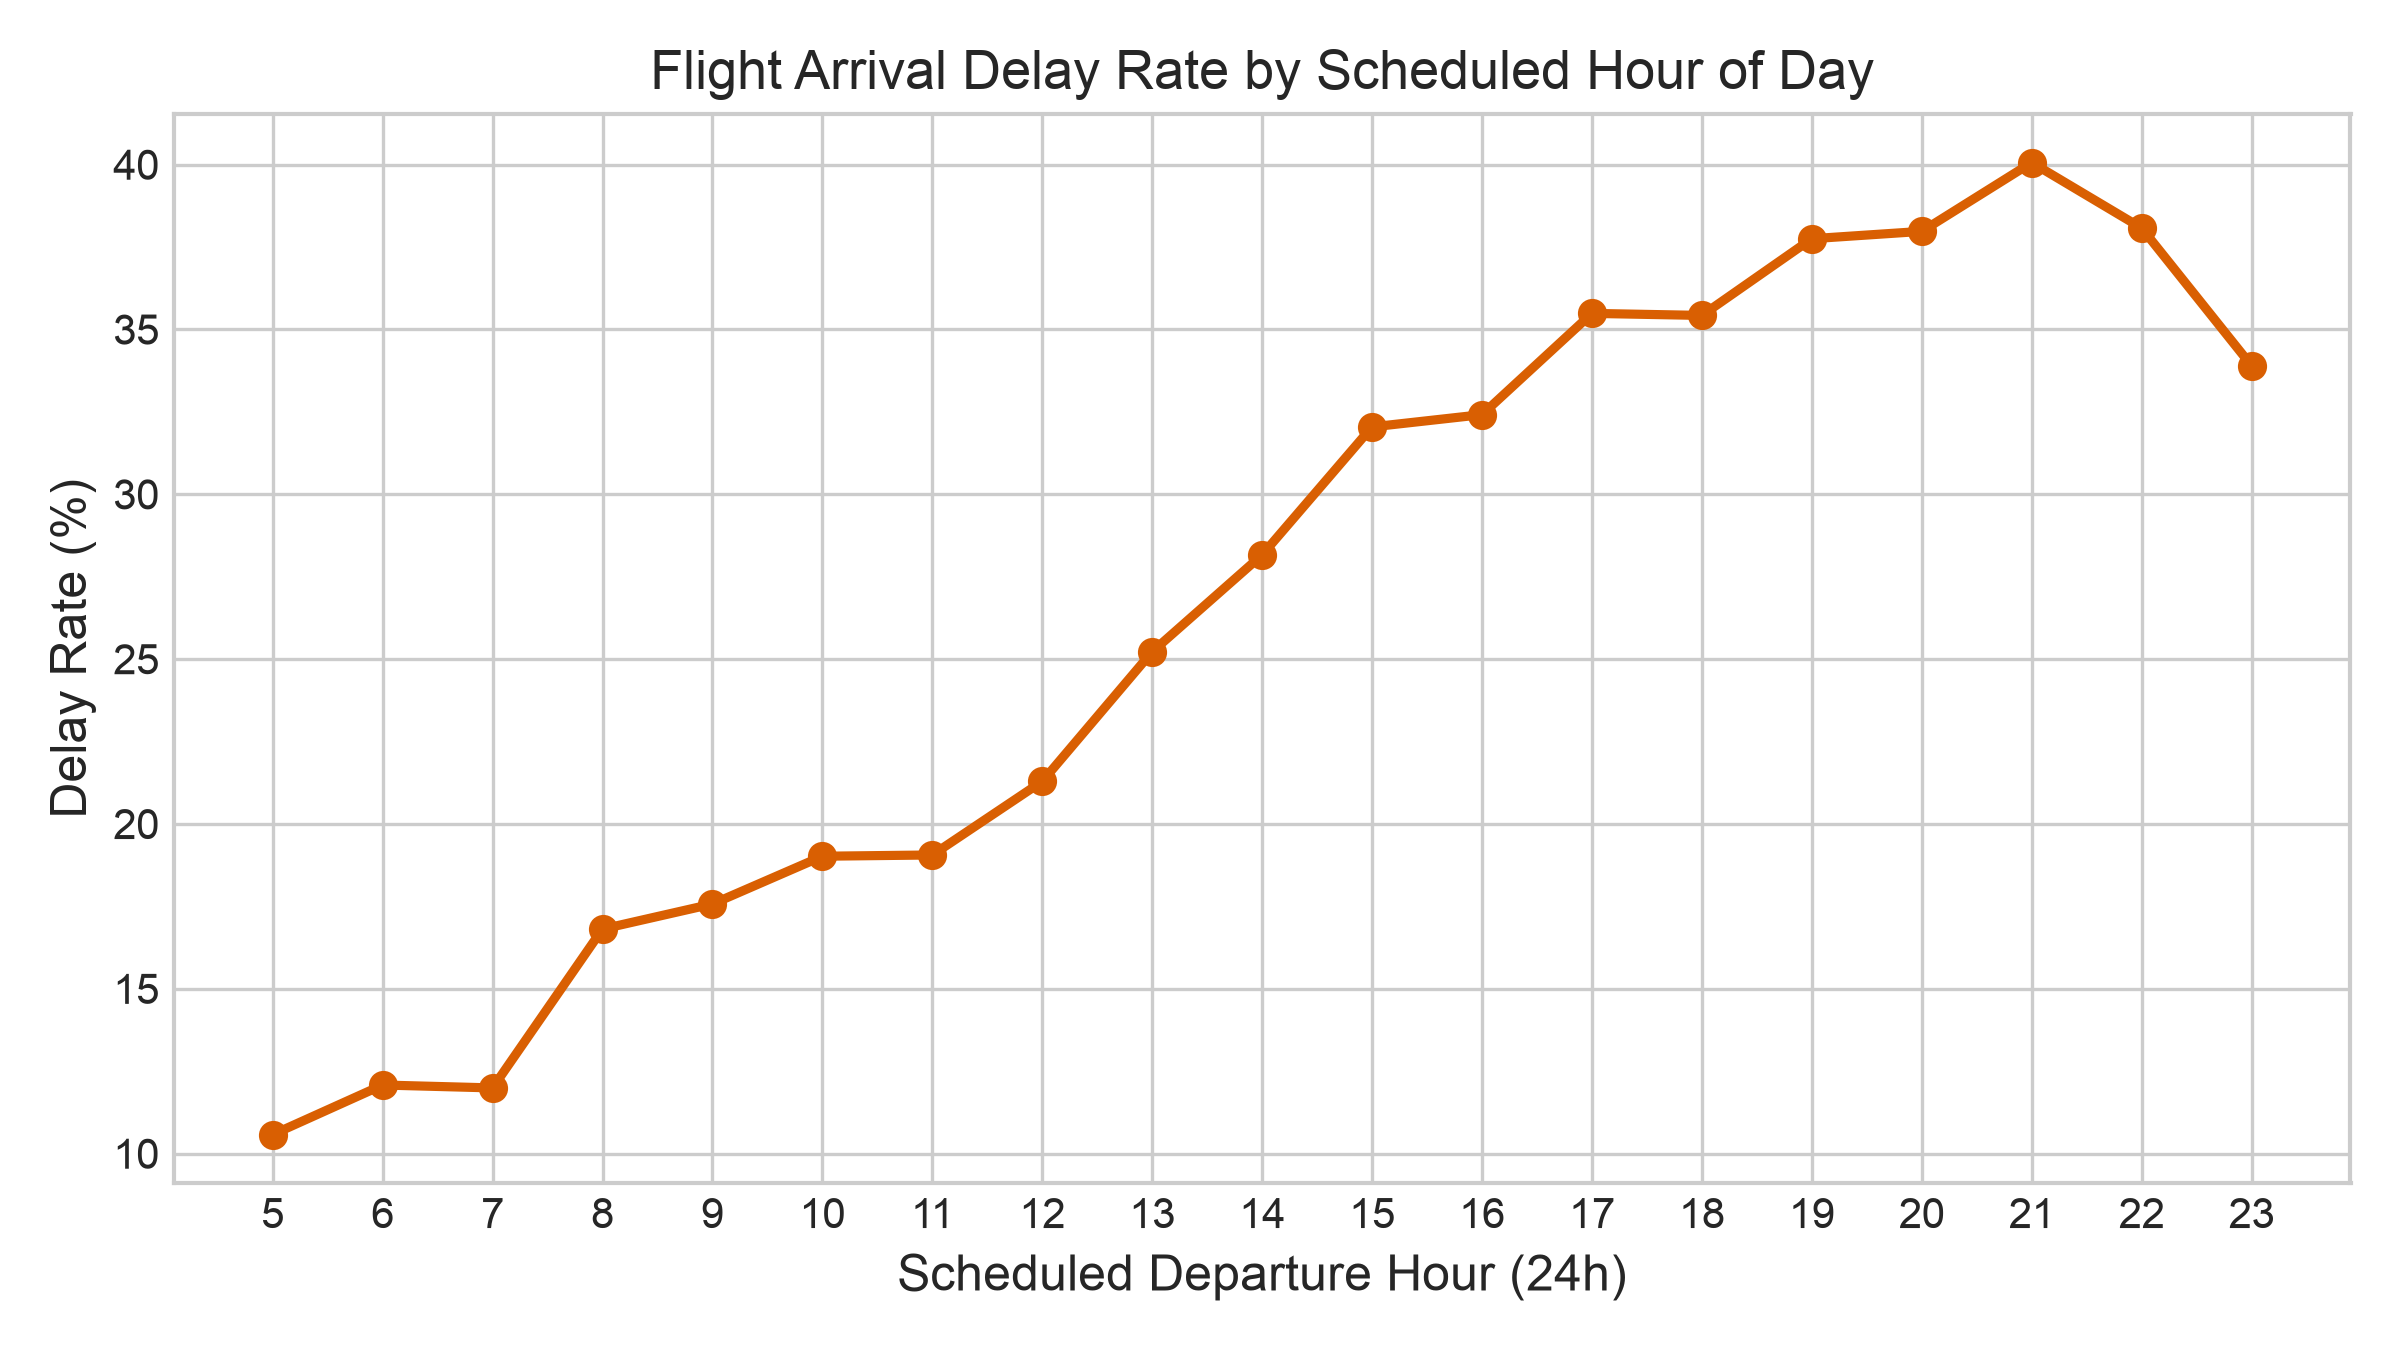
\includegraphics[width=\columnwidth]{../../results/figures/eda_delay_by_hour.png}\caption{Delay variation by scheduled departure hour in the fitted training population. Descriptive associations are not causal. Source: saved project EDA.}\label{fig:eda}\end{figure}
\section{Experimental Protocol}
\begin{table}[t]\caption{Chronological roles and available labeled rows. Dates are inclusive, 2013.}\label{tab:split}\centering\footnotesize\begin{tabular}{lrrr}\toprule Role & Dates & Candidate & Usable\\\midrule Training & Jan 1--Sep 12 & 228,299 & 227,520\\ Fusion/calibration fit & Sep 13--Oct 1 & 17,398 & 16,434\\ Selection & Oct 2--Oct 19 & 16,451 & 15,765\\ Threshold selection & Oct 20--Nov 6 & 16,617 & 15,646\\ Test & Nov 7--Dec 31 & 48,581 & 48,581\\\bottomrule\end{tabular}\end{table}
Table~\ref{tab:split} gives date-preserving blocks. At each fitting or policy boundary, labels not yet released or invalid for historical availability are purged. The training prevalence before purging is 25.91\%; the three usable development blocks have 11.96\%, 18.75\%, and 17.38\% positives, respectively, and test has 26.86\%. Prevalence shift makes threshold and calibration transfer difficult.

Four expanding training-only folds with 30-date forward holdouts tune candidate feature families and classical-model parameters. Each fold refits preprocessing. A subsequent selection block chooses feature family by raw average precision (AP); final base estimators are fit on available training labels. Logistic regression selects historical rates and demand; XGBoost selects cyclic schedule and demand. The MLP uses the XGBoost numeric selection. Calibration candidates are fit on the first development block and identity, sigmoid, or isotonic is selected by Brier loss on the second. Fusion is also fit on the first block, so hybrid calibrator fitting uses predictions from the same data used to fit fusion; this can increase optimism even though calibration selection uses later dates. Thresholds are selected on the third block and frozen before test.

Test outputs had already been inspected during review. Consequently this is a corrected retrospective reevaluation, not a pristine external test, even though the documented final selection decisions use development blocks. The saved run used seed 42, 200 whole-date bootstrap replicates, CPU neural training, Python 3.12.5, PyTorch 2.14.1, XGBoost 3.4.1 and scikit-learn 1.9.1 as recorded in run metadata. The saved hash of the concatenated source files matches the recorded base Git revision; the current source hash differs because of import cleanups in two files. The run records a dirty working tree, so the hash does not establish the state of files outside its scope. We did not rerun training.
\section{Models and Hybrid Architecture}
Logistic regression minimizes binary log loss with L2 regularization; selected $C=0.03$ and no class weighting. XGBoost fits additive trees on logistic loss, with selected 42 trees, depth 3, learning rate 0.06, minimum child weight 100 and leaf L2 penalty 5. These are selected configurations, not claims of a globally optimal search.

The MLP learns carrier, origin, and destination embeddings of 16, 16 and 32 dimensions, concatenates them with selected numeric features, and passes them through dense layers of 128, 64 and 32 units, each with batch normalization, ReLU and dropout 0.2. A final linear unit produces logit $z$ and probability $\sigma(z)$. Binary cross-entropy with logits is minimized with Adam, learning rate $10^{-3}$, weight decay $10^{-4}$, batch size 512 and 15 fixed epochs. Development monitoring did not select the checkpoint. Embedding lookup gives a trainable vector for each category, not a validated semantic airport map.

The deployed hybrid receives XGBoost raw margin $z_T$ and MLP logit $z_N$ and computes
\begin{equation}
 p_H=\sigma(b+w_T z_T+w_N z_N),\quad \sigma(z)=(1+e^{-z})^{-1}.
\label{eq:fusion}\end{equation}
The two coefficients and intercept are learned by L2-regularized logistic regression on the first development block, using base predictions from models fit on earlier training data. This is a fixed linear logit fusion, not a sample-dependent gating network. Isotonic calibration was selected for its output. Trees can partition tabular values while embeddings learn category representations; combining them might improve prediction if their errors contain useful complementary information. Neither independence nor improvement follows from Eq.~\eqref{eq:fusion}. A standalone tabular ResNet is implemented and trained in small exploratory ablations; it is not the final hybrid's neural branch.
\section{Evaluation and Results}
AP summarizes the precision--recall ranking as a recall-weighted sum, not trapezoidal PR area. ROC-AUC also assesses ranking; Brier loss $N^{-1}\sum_i(p_i-y_i)^2$ assesses probability error and combines calibration and resolution. Table~\ref{tab:results} uses raw probabilities for AP/AUC and selected probability outputs for Brier and threshold metrics. Constant-prior AP equals test prevalence; at its 0.5 threshold it produces no alerts, so precision is undefined.
\begin{table*}[t]\caption{Retrospective test results, $N=48{,}581$, prevalence 0.2686. AP and AUC use raw scores; Brier and operating metrics use selected probability scale.}\label{tab:results}\centering\small\begin{tabular}{lrrrrrrrl}\toprule Model & AP & AUC & Brier & Threshold & Precision & Recall & Alerts & Calibration\\\midrule Logistic regression & .3200 & .5797 & .2396 & .091 & .3399 & .1967 & 7,550 & identity\\ XGBoost & .3722 & .6367 & .1910 & .206 & .3449 & .6774 & 25,622 & identity\\ Embedding MLP & .3936 & .6506 & .2017 & .063 & .3195 & .8304 & 33,913 & identity\\ Hybrid & .3557 & .6239 & .2091 & .143 & .3495 & .4582 & 17,106 & isotonic\\ Constant training prior & .2686 & .5000 & .1965 & .500 & -- & .0000 & 0 & constant\\\bottomrule\end{tabular}\end{table*}
The MLP has the highest raw AP and recall among evaluated models, but generates many alerts; XGBoost has the best Brier loss and improves on the constant prior's 0.1965. The hybrid trails both components in raw AP and AUC and has worse Brier than either. Its isotonic test AP is 0.3407, distinct from raw AP because ties can change ranking. Hybrid raw Brier is 0.2094 versus 0.2091 after selected calibration: a small retrospective difference does not establish superior calibration. Reliability curves show substantial underprediction in many test bins (Fig.~\ref{fig:cal}).

The configured development objective was maximum recall at 70\% precision with at least 100 alerts; this project-chosen target was not met for any model. The declared fallback maximized development $F_1$ subject to the same support. Test precision is about 32--35\%, not 70\%. These operating points are conditional on the selected probability scale, support and prevalence; they should not be interpreted as operational guarantees.

Whole-date bootstrap 95\% intervals for raw AP are [0.3188, 0.4367] for XGBoost, [0.3295, 0.4639] for MLP and [0.3031, 0.4199] for hybrid. These 200-replicate intervals describe date resampling of this test, not independent future years or a paired significance test. For XGBoost, selected-score AP is 0.4202 at EWR ($n=17{,}099$, prevalence 28.73\%), 0.3201 at JFK ($n=15{,}866$, 25.63\%) and 0.3491 at LGA ($n=15{,}616$, 26.05\%). Saved carrier, hour and date slices also permit inspection; differing prevalence and small groups limit comparisons. No claim of uniform subgroup performance is warranted.
\begin{figure*}[t]\centering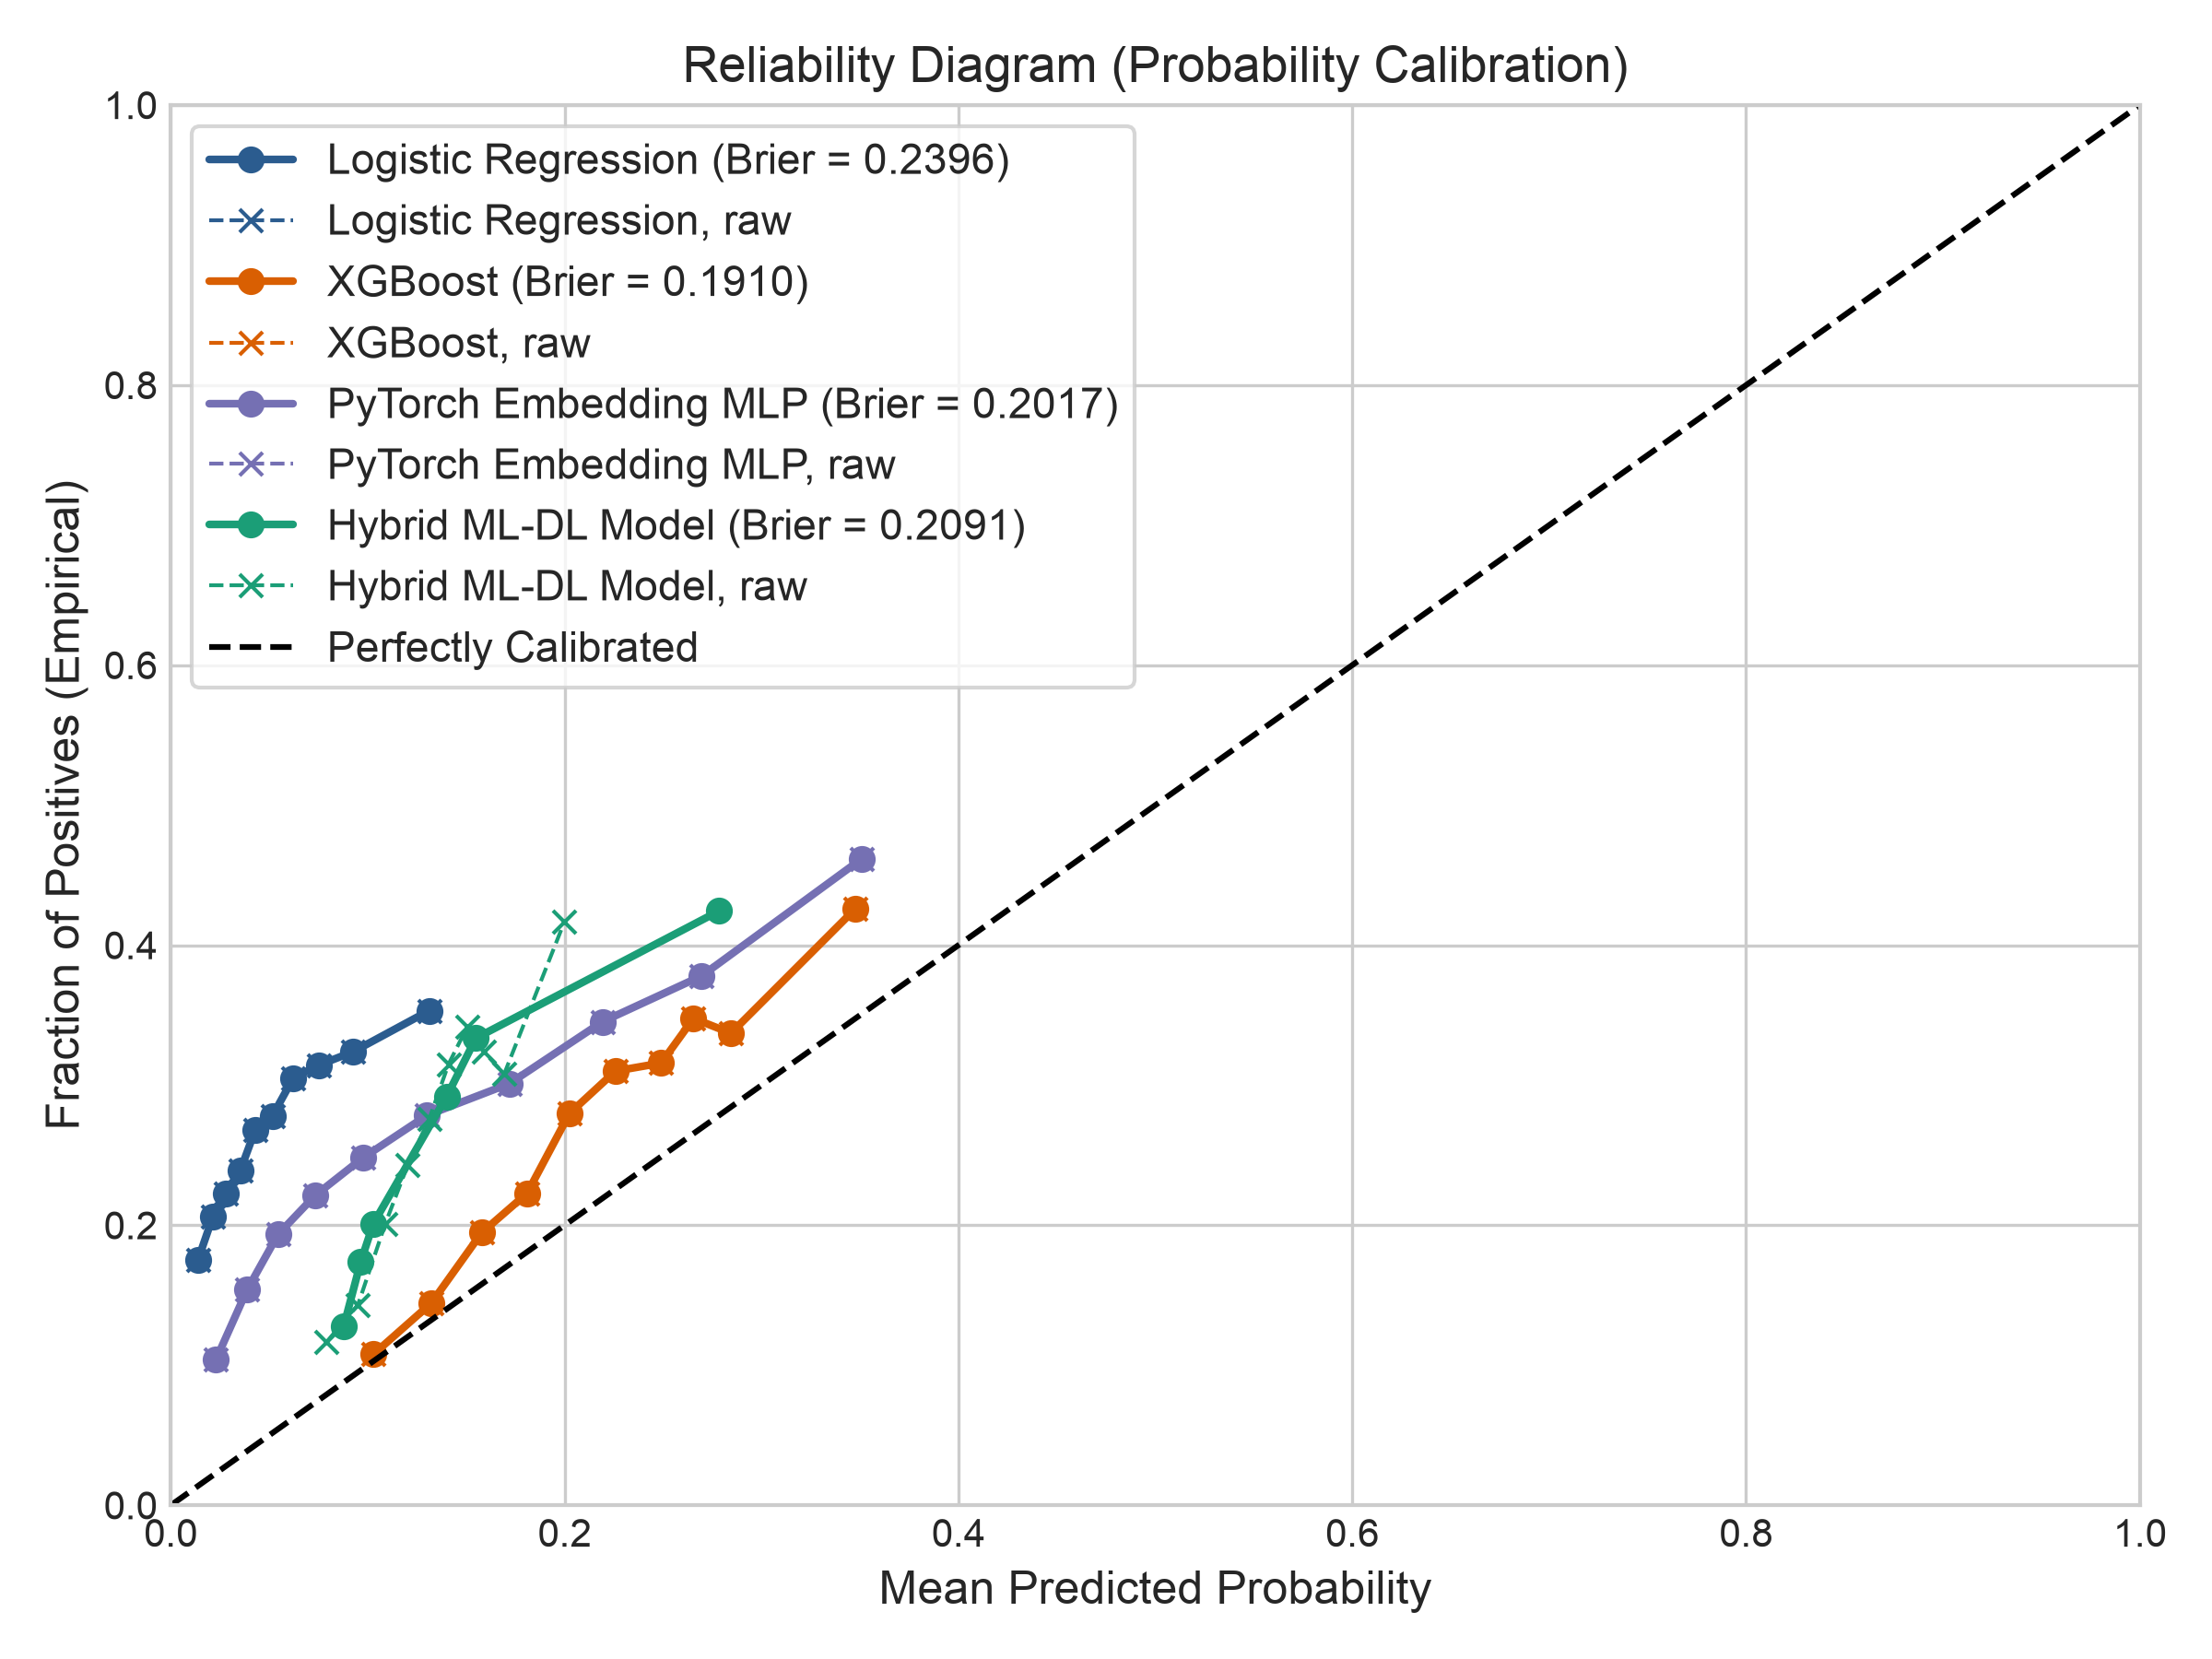
\includegraphics[width=0.72\textwidth]{../../results/figures/calibration_curves.png}\caption{Saved test reliability curves for raw and selected outputs. Bin frequencies and selection under distribution shift affect interpretation.}\label{fig:cal}\end{figure*}
\section{Ablation Evidence}
Feature ablations fit fixed configurations and evaluate on the selection block: XGBoost AP falls from 0.3286 for schedule/calendar to 0.2895 with history and 0.2866 with scheduled demand added to that configuration; logistic regression gives 0.3388, 0.3349 and 0.3392, respectively. The frozen-history reference gives 0.3074 and 0.3348. Feature sets and model fitting differ from final selection; these are exploratory development results, not causal feature effects or test comparisons.

The hybrid-paradigm study uses 15,765 selection-block observations. Although the saved table labels the neural output ``Deep ResNet,'' the pipeline passes the trained MLP logits. XGBoost, MLP and equal probability averaging achieve AP 0.3397, 0.2938 and 0.3075 and Brier 0.1427, 0.1517 and 0.1447. A separate fitted fusion achieves AP 0.3374 and Brier 0.1419 \emph{on the same block used to fit its coefficients} ($w_T=1.289$, $w_N=0.060$, $b=0.473$). These are exploratory in-sample scores for that ablation, not independent validation or coefficients of the final hybrid.

Architecture and regularization studies draw 12,000 fitting rows and 4,000 selection rows with seed 42 and train three epochs. Shallow MLP, three-layer MLP, one-block ResNet and three-block ResNet yield AP 0.2985, 0.3318, 0.3081 and 0.3183. Width, depth, block type and capacity change together; training budget is short and initialization varies, so the comparison cannot isolate skip connections or establish a best architecture. For two-block ResNets, no regularization, dropout only (0.3), weight decay only ($10^{-3}$), and dropout 0.2 plus decay $10^{-4}$ yield AP 0.3124, 0.3131, 0.2907 and 0.2906. With one seed and changing strengths, these do not prove regularization prevents overfitting or isolate each effect. None was the saved final MLP training protocol.
\section{Schedule Sensitivity and Limitations}
The historical app scores flights and considers departure-time shifts while preserving scheduled duration and rebuilding time and demand features. The simulator uses XGBoost with its selected probability treatment and shifts one focal flight against a fixed background timetable; the historical information set remains fixed. The resulting change in model probability is an offline sensitivity, not an observed or causal effect of rescheduling. Slots, gates, rotations, crew, passenger connections and reactions of other flights are not modeled.

One year and three origins restrict temporal and geographic transfer. Missing outcomes can induce selection bias; weather, operational capacity and aircraft rotations are absent. Timetable availability, reconstructed arrival clocks and 24-hour release lag are assumptions; a versioned live feed is needed to validate them. Daily outcome replay is not a frozen-history evaluation. The retrospectively inspected test and incomplete provenance of the dirty working tree further weaken external claims. To establish hybrid value, future work should use fresh chronological periods or airports, matched component tuning, independent or cross-fitted fusion and calibration data, paired date-block comparisons, and actual availability logs. A prospective operational evaluation would additionally need feasible interventions and causal design.
\section{Conclusion}
The embedding MLP ranked delays best in this saved retrospective test, while XGBoost produced the lowest Brier loss. The learned XGBoost--MLP hybrid did not improve on its components in the reported comparison. The implementation illustrates a defensible availability-aware hypothesis and offline sensitivity workflow, with material limitations that prevent operational or causal claims.
\appendices
\section{Reproduction and Verification Notes}
The repository provides a pinned download, a seeded pipeline, artifact verification and tests. The raw CSV and compatible environment are needed for full replay. The source hash matches the recorded base revision; later hashed-file changes are import cleanups, while other dirty-tree contents are unknown. Full retraining, artifact replay and tests were not run for this report. Build and reproduction commands accompany the source.
\bibliographystyle{IEEEtran}
\bibliography{T001_Phase2_verified}
\clearpage
\onecolumn
\section*{Team T001 Contribution Matrix}
The following Phase 2 responsibilities are based on the team-supplied work split. They describe areas of responsibility rather than independently audited code ownership.
\begin{center}
\renewcommand{\arraystretch}{1.5}
\begin{tabular}{@{}>{\raggedright\arraybackslash}p{0.20\textwidth}>{\raggedright\arraybackslash}p{0.16\textwidth}>{\raggedright\arraybackslash}p{0.58\textwidth}@{}}
\toprule
\textbf{Member} & \textbf{Enrollment} & \textbf{Phase 2 responsibility} \\
\midrule
Sarthak Mishra & 2401010421 & Team lead; deep learning and hybrid architecture, model definitions, training routines and configuration. \\
Shane & 2401020062 & Data pipeline, chronological splitting, timestamp handling and information-availability safeguards. \\
Shitanshu Tiwari & 2401010440 & XGBoost modeling, temporal feature engineering and forward model-selection experiments. \\
Preetish Ubhrani & 2401020050 & Probability calibration, evaluation metrics and operational decision thresholds. \\
Kshitiz & 2401010242 & Ablation studies, Streamlit demonstrator, artifact verification and demonstration support. \\
\bottomrule
\end{tabular}
\end{center}
\end{document}
